% =============================================================================
% Standalone Plots for Analysis and Results Section
% Compile with: pdflatex plots.tex
% =============================================================================

\documentclass[tikz]{standalone}
\usepackage{pgfplots}
\usepackage{pgfplotstable}
\pgfplotsset{compat=1.18}

\begin{document}

% Plot 1: Performance Metrics Across K-Fold Configurations
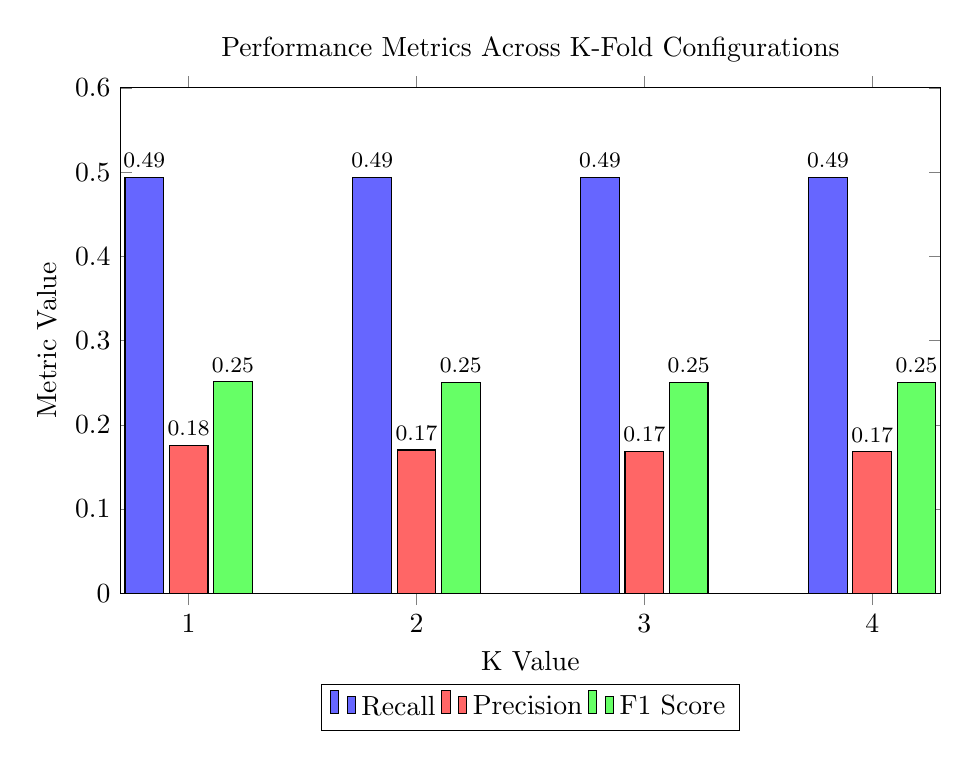
\begin{tikzpicture}
\begin{axis}[
    ybar,
    width=12cm,
    height=8cm,
    xlabel={K Value},
    ylabel={Metric Value},
    ymin=0, ymax=0.6,
    xtick={1,2,3,4},
    legend style={at={(0.5,-0.18)}, anchor=north, legend columns=3},
    bar width=14pt,
    nodes near coords,
    nodes near coords align={vertical},
    every node near coord/.append style={font=\footnotesize},
    title={Performance Metrics Across K-Fold Configurations},
]
\addplot[fill=blue!60] coordinates {(1,0.4933) (2,0.4933) (3,0.4933) (4,0.4933)};
\addplot[fill=red!60] coordinates {(1,0.1756) (2,0.1701) (3,0.1684) (4,0.1678)};
\addplot[fill=green!60] coordinates {(1,0.2509) (2,0.2503) (3,0.2501) (4,0.2500)};
\legend{Recall, Precision, F1 Score}
\end{axis}
\end{tikzpicture}

\newpage

% Plot 2: Recall by Story (K=1)
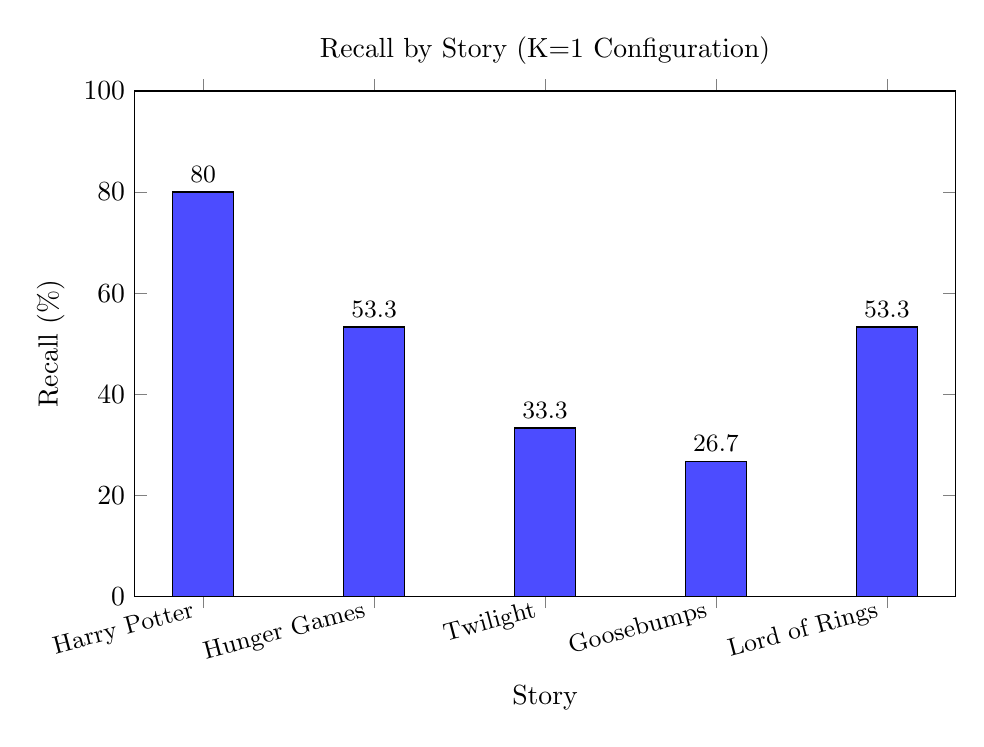
\begin{tikzpicture}
\begin{axis}[
    ybar,
    width=12cm,
    height=8cm,
    xlabel={Story},
    ylabel={Recall (\%)},
    ymin=0, ymax=100,
    symbolic x coords={Harry Potter, Hunger Games, Twilight, Goosebumps, Lord of Rings},
    xtick=data,
    x tick label style={rotate=15, anchor=east, font=\small},
    bar width=22pt,
    nodes near coords,
    nodes near coords align={vertical},
    every node near coord/.append style={font=\small},
    title={Recall by Story (K=1 Configuration)},
]
\addplot[fill=blue!70] coordinates {
    (Harry Potter,80.0) 
    (Hunger Games,53.3) 
    (Twilight,33.3) 
    (Goosebumps,26.7) 
    (Lord of Rings,53.3)
};
\end{axis}
\end{tikzpicture}

\newpage

% Plot 3: Precision by Story (K=1)
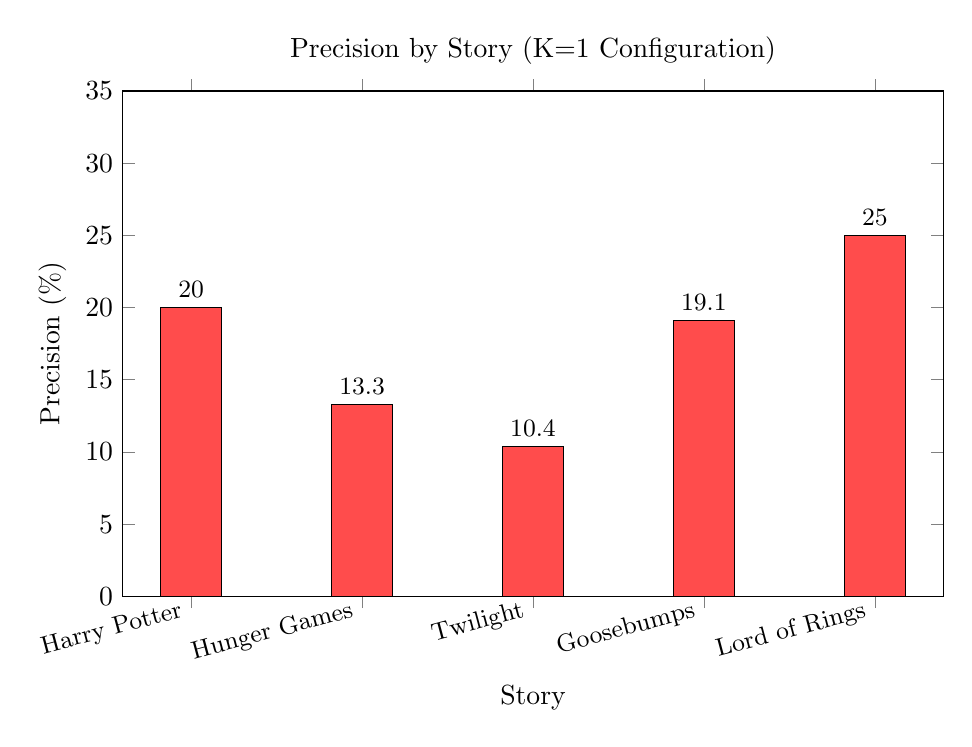
\begin{tikzpicture}
\begin{axis}[
    ybar,
    width=12cm,
    height=8cm,
    xlabel={Story},
    ylabel={Precision (\%)},
    ymin=0, ymax=35,
    symbolic x coords={Harry Potter, Hunger Games, Twilight, Goosebumps, Lord of Rings},
    xtick=data,
    x tick label style={rotate=15, anchor=east, font=\small},
    bar width=22pt,
    nodes near coords,
    nodes near coords align={vertical},
    every node near coord/.append style={font=\small},
    title={Precision by Story (K=1 Configuration)},
]
\addplot[fill=red!70] coordinates {
    (Harry Potter,20.0) 
    (Hunger Games,13.3) 
    (Twilight,10.4) 
    (Goosebumps,19.1) 
    (Lord of Rings,25.0)
};
\end{axis}
\end{tikzpicture}

\newpage

% Plot 4: F1 Score by Story (K=1)
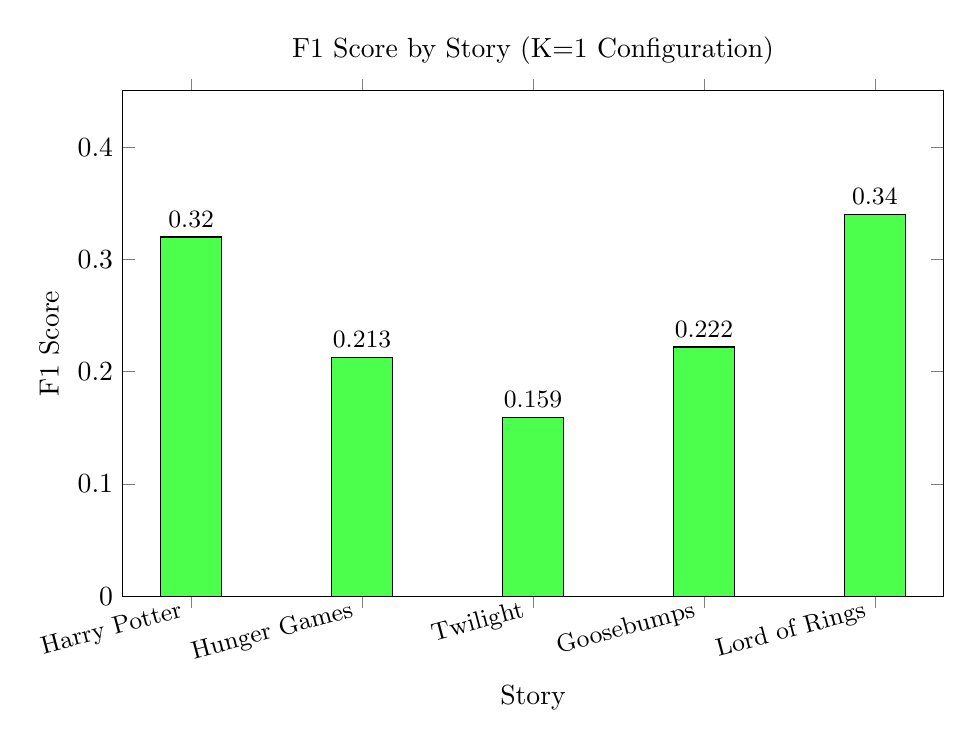
\begin{tikzpicture}
\begin{axis}[
    ybar,
    width=12cm,
    height=8cm,
    xlabel={Story},
    ylabel={F1 Score},
    ymin=0, ymax=0.45,
    symbolic x coords={Harry Potter, Hunger Games, Twilight, Goosebumps, Lord of Rings},
    xtick=data,
    x tick label style={rotate=15, anchor=east, font=\small},
    bar width=22pt,
    nodes near coords,
    nodes near coords align={vertical},
    every node near coord/.append style={font=\small, /pgf/number format/precision=3},
    title={F1 Score by Story (K=1 Configuration)},
]
\addplot[fill=green!70] coordinates {
    (Harry Potter,0.320) 
    (Hunger Games,0.213) 
    (Twilight,0.159) 
    (Goosebumps,0.222) 
    (Lord of Rings,0.340)
};
\end{axis}
\end{tikzpicture}

\newpage

% Plot 5: Recall by Error Category
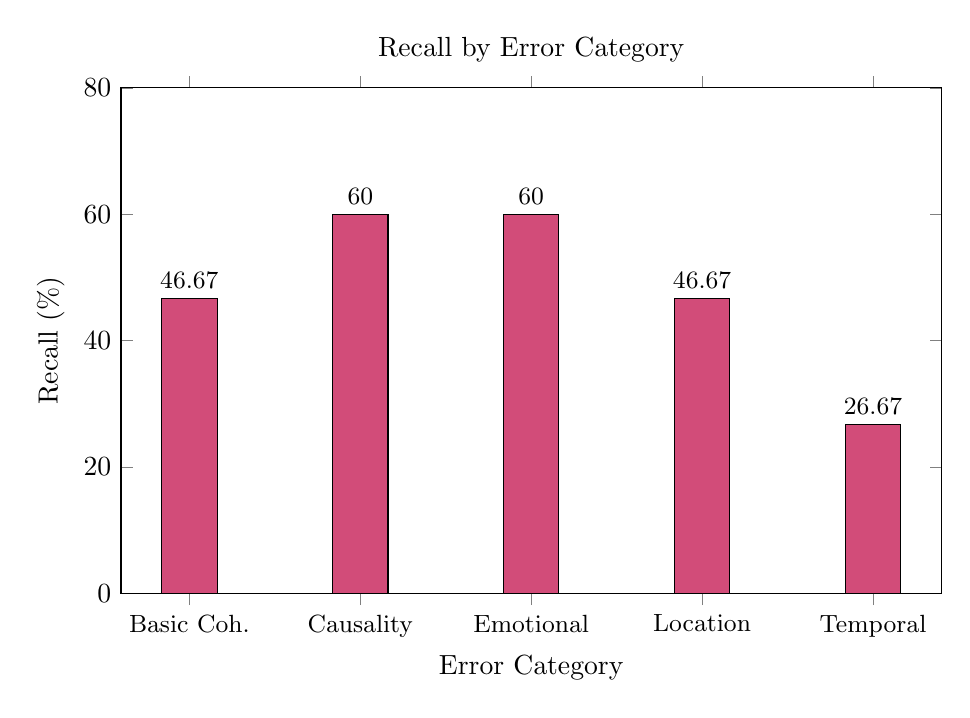
\begin{tikzpicture}
\begin{axis}[
    ybar,
    width=12cm,
    height=8cm,
    xlabel={Error Category},
    ylabel={Recall (\%)},
    ymin=0, ymax=80,
    symbolic x coords={Basic Coh., Causality, Emotional, Location, Temporal},
    xtick=data,
    x tick label style={font=\small},
    bar width=20pt,
    nodes near coords,
    nodes near coords align={vertical},
    every node near coord/.append style={font=\small},
    title={Recall by Error Category},
]
\addplot[fill=purple!70] coordinates {
    (Basic Coh.,46.67) 
    (Causality,60.0) 
    (Emotional,60.0) 
    (Location,46.67) 
    (Temporal,26.67)
};
\end{axis}
\end{tikzpicture}

\newpage

% Plot 6: Precision-Recall Scatter Plot
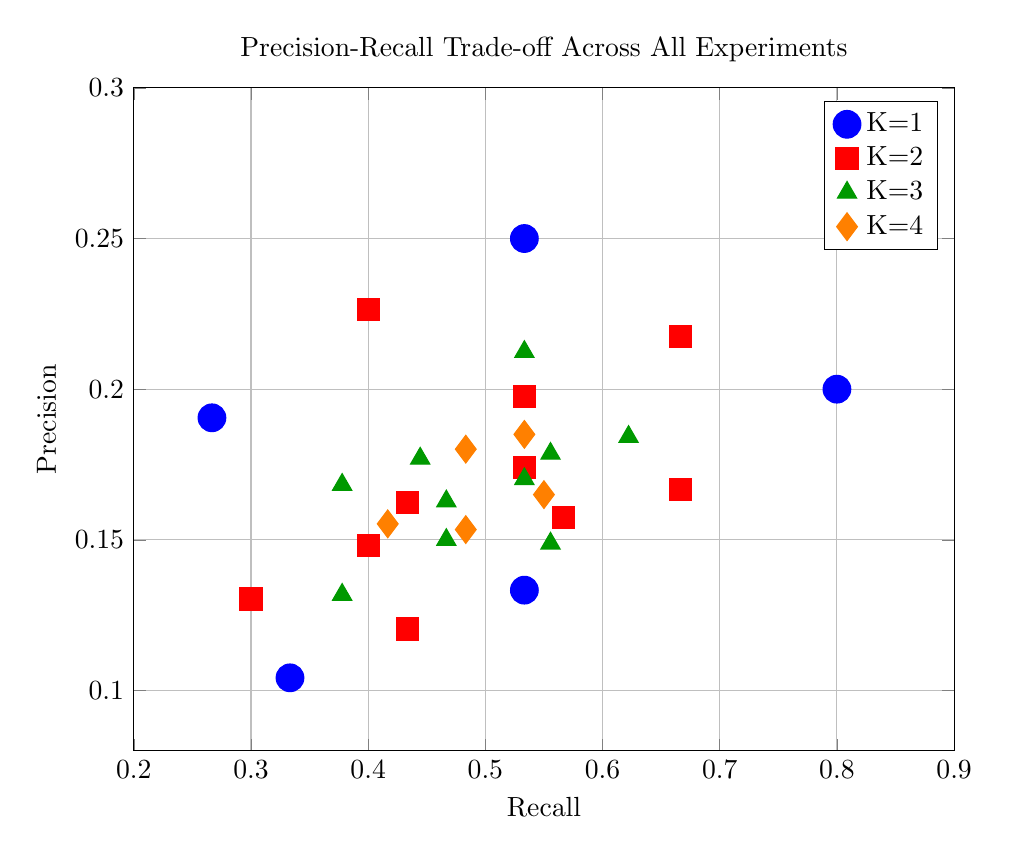
\begin{tikzpicture}
\begin{axis}[
    width=12cm,
    height=10cm,
    xlabel={Recall},
    ylabel={Precision},
    xmin=0.2, xmax=0.9,
    ymin=0.08, ymax=0.30,
    legend style={at={(0.98,0.98)}, anchor=north east},
    mark size=4pt,
    grid=both,
    minor grid style={gray!25},
    major grid style={gray!50},
    title={Precision-Recall Trade-off Across All Experiments},
]
% K=1 points
\addplot[only marks, mark=*, blue, mark size=5pt] coordinates {
    (0.80,0.20) (0.5333,0.1333) (0.3333,0.1042) (0.2667,0.1905) (0.5333,0.25)
};
% K=2 points
\addplot[only marks, mark=square*, red, mark size=4pt] coordinates {
    (0.6667,0.1667) (0.5667,0.1574) (0.5333,0.1975) (0.6667,0.2174)
    (0.4333,0.1204) (0.40,0.1481) (0.5333,0.1739)
    (0.30,0.1304) (0.4333,0.1625) (0.40,0.2264)
};
% K=3 points
\addplot[only marks, mark=triangle*, green!60!black, mark size=4pt] coordinates {
    (0.5556,0.1488) (0.5333,0.1702) (0.6222,0.1842) (0.4667,0.1628) (0.5556,0.1786)
    (0.5333,0.2124) (0.3778,0.1318) (0.4667,0.15) (0.4444,0.177) (0.3778,0.1683)
};
% K=4 points
\addplot[only marks, mark=diamond*, orange, mark size=5pt] coordinates {
    (0.4833,0.1534) (0.55,0.165) (0.5333,0.185) (0.4833,0.1801) (0.4167,0.1553)
};
\legend{K=1, K=2, K=3, K=4}
\end{axis}
\end{tikzpicture}

\newpage

% Plot 7: True Positives and False Positives by Story
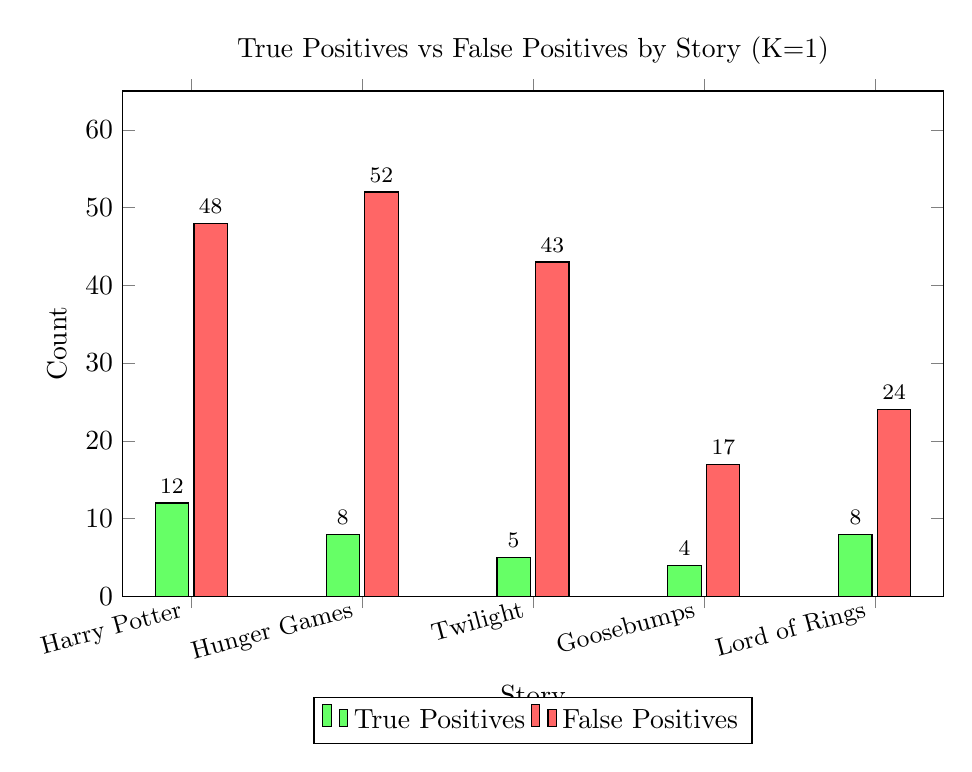
\begin{tikzpicture}
\begin{axis}[
    ybar,
    width=12cm,
    height=8cm,
    xlabel={Story},
    ylabel={Count},
    ymin=0, ymax=65,
    symbolic x coords={Harry Potter, Hunger Games, Twilight, Goosebumps, Lord of Rings},
    xtick=data,
    x tick label style={rotate=15, anchor=east, font=\small},
    legend style={at={(0.5,-0.20)}, anchor=north, legend columns=2},
    bar width=12pt,
    nodes near coords,
    nodes near coords align={vertical},
    every node near coord/.append style={font=\footnotesize},
    title={True Positives vs False Positives by Story (K=1)},
]
\addplot[fill=green!60] coordinates {
    (Harry Potter,12) 
    (Hunger Games,8) 
    (Twilight,5) 
    (Goosebumps,4) 
    (Lord of Rings,8)
};
\addplot[fill=red!60] coordinates {
    (Harry Potter,48) 
    (Hunger Games,52) 
    (Twilight,43) 
    (Goosebumps,17) 
    (Lord of Rings,24)
};
\legend{True Positives, False Positives}
\end{axis}
\end{tikzpicture}

\newpage

% Plot 8: F1 Score Comparison Across K Values
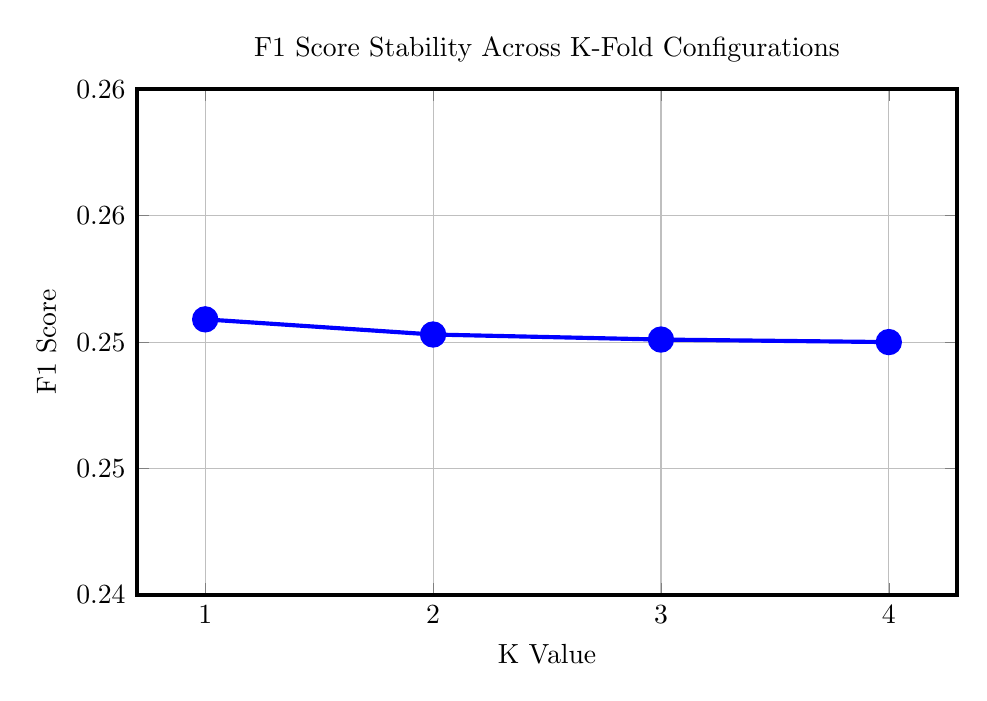
\begin{tikzpicture}
\begin{axis}[
    width=12cm,
    height=8cm,
    xlabel={K Value},
    ylabel={F1 Score},
    ymin=0.24, ymax=0.26,
    xtick={1,2,3,4},
    mark=*,
    mark size=4pt,
    line width=1.5pt,
    title={F1 Score Stability Across K-Fold Configurations},
    grid=both,
]
\addplot[blue, mark=*] coordinates {
    (1,0.2509) (2,0.2503) (3,0.2501) (4,0.2500)
};
\end{axis}
\end{tikzpicture}

\newpage

% Plot 9: Detection Rate by Error Category and Story (Heatmap style)
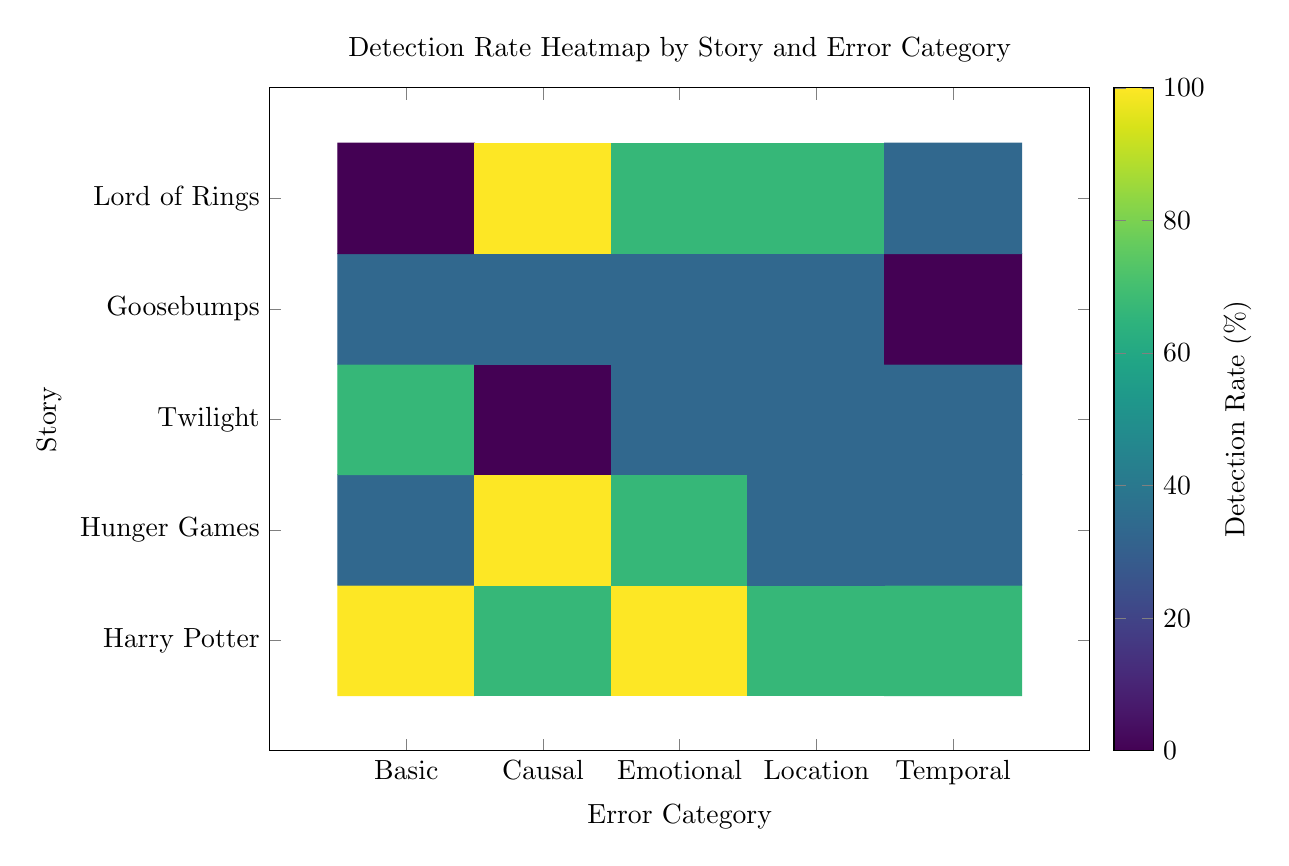
\begin{tikzpicture}
\begin{axis}[
    colormap/viridis,
    colorbar,
    colorbar style={
        ylabel={Detection Rate (\%)},
    },
    width=12cm,
    height=10cm,
    xlabel={Error Category},
    ylabel={Story},
    xtick={0,1,2,3,4},
    xticklabels={Basic, Causal, Emotional, Location, Temporal},
    ytick={0,1,2,3,4},
    yticklabels={Harry Potter, Hunger Games, Twilight, Goosebumps, Lord of Rings},
    title={Detection Rate Heatmap by Story and Error Category},
    point meta min=0,
    point meta max=100,
]
\addplot[
    matrix plot*,
    mesh/cols=5,
    point meta=explicit,
] table[meta=C] {
x y C
0 0 100
1 0 66.67
2 0 100
3 0 66.67
4 0 66.67
0 1 33.33
1 1 100
2 1 66.67
3 1 33.33
4 1 33.33
0 2 66.67
1 2 0
2 2 33.33
3 2 33.33
4 2 33.33
0 3 33.33
1 3 33.33
2 3 33.33
3 3 33.33
4 3 0
0 4 0
1 4 100
2 4 66.67
3 4 66.67
4 4 33.33
};
\end{axis}
\end{tikzpicture}

\newpage

% Plot 10: Cumulative Performance by K
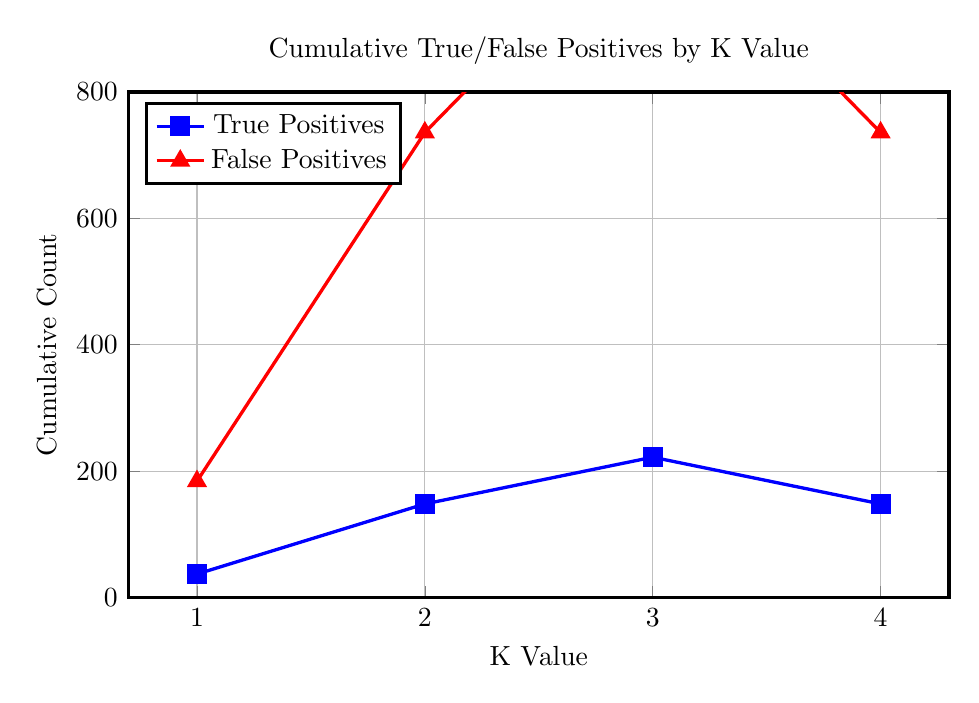
\begin{tikzpicture}
\begin{axis}[
    width=12cm,
    height=8cm,
    xlabel={K Value},
    ylabel={Cumulative Count},
    ymin=0, ymax=800,
    xtick={1,2,3,4},
    legend style={at={(0.02,0.98)}, anchor=north west},
    mark size=3pt,
    line width=1.2pt,
    title={Cumulative True/False Positives by K Value},
    grid=both,
]
\addplot[blue, mark=square*] coordinates {(1,37) (2,148) (3,222) (4,148)};
\addplot[red, mark=triangle*] coordinates {(1,184) (2,736) (3,1104) (4,736)};
\legend{True Positives, False Positives}
\end{axis}
\end{tikzpicture}

\end{document}
